\documentclass[aspectratio=169]{beamer}

\usetheme{vega}



\title{}
\subtitle{Влияние макроэкономических показателей страны на уровень индивидуального благополучия граждан}
\author{Заостровский Всеволод, Сулейманов Асхаб, Черепахин Иван}
\supervisor{Станкевич Иван Павлович}
\institute{Vega Institute Foundation, Мехмат МГУ}

\date{}

\usepackage[]{lipsum}
\begin{document}
\maketitle

    

    

\begin{frame}{1.Введение}
   В чём смысл существования государства? Этим вопросом задавались тысячи мыслителей на протяжении всей истории человечества. Более того, очень многие из них были твёрдо убеждены в том, что именно им удалось услышать голос Истины, хотя, конечно, сценарий при котором одна и та же Истина, вмещающая в себя сущность государства, одновременно описывается миллионами эпитетов, аллегорий и фразеологизмов, колеблющихся от ’самого холодного из всех холодных чудовищ’ до ’намордника для усмирения плотоядного животного, называющегося человеком’, кажется, по меньшей мере, весьма и весьма маловероятным. Мы, конечно, не ставим задачи углубиться в тысячелетнюю историю этой дискуссии, и отвечаем на этот вопрос до наивности бесхитростно: смысл государства, равно как и всякого изобретения человечества, состоит в привнесении счастья в печальное настоящее нашего рода. 
\hfill \break
\hfill \break
   Однако, далеко не все творения покорно следуют замыслам своих создателей, потому интересно разобраться в том, каких побед человечеству удалось достичь на этом поприще и в каком направлении следует двигаться дальше.
     
 \end{frame}

\begin{frame}{1.Введение}
   Одним из главных вопросов современной дискуссии является: что же влияет на уровень счастья? Многие убеждены, в том числе и среди видных мыслителей, что счастье в первую очередь зависит от субъективных, мировозренческих, ценностных, идеологических, психологических факторах, нежели чем от объективных факторов по типу благосостояния. Иные же считают, что главную роль играет не абсолютный уровень богатсва общетсва, а скорее относительный уровень. Например, человек оценивает свою успешность, а соответсвенно и удовлетворенность от жизни, сравнивая себя с другими членами общетства. Приверженцы таких идеи, пытаясь доказать свою правоту, обычно приводят частные примеры, которые, кстати говоря, весьма убедительны и способны склонить колеблющихся в дискуссии в свою сторону. Приведём часть из них, чтоб продемонстрировать всю серьёзность изучаемого вопроса. 
\end{frame}

\begin{frame}{1.Введение}
   Сообщество World Happiness Report введем постоянный отчет субъективного восприятия людей уровня своего счастья по странам мира. Откуда мы можем получать весьма занимательные факты. Например, такая высокоразвитая страна как Южная Корея, занимающая лидирующие позиции в микроэлектронике, машиностроении, судостроении, атомной энегетике и т.д., по уровню счатья занимает лишь 55 место, на одном уровне с Молдавией, имеющая 100 место по ВВП на душу ППС. Это согласуется и с одним из самых высоких уровней самоубийтсв на душу населения(12 место в мире). И в то же время Узбекистан имеет относительно высокий уровень счастья, занимая 47 место, имея 131 место по ВВП на душу ППС. 
   
   \begin{figure} \label{hompic}
            \centering
            
\includegraphics[scale=0.32]{Union1.png}
    \end{figure}

\end{frame}

\begin{frame}{1.Введение}
   Мы же попытаемся показать, что макроэкономические достижения стран всё же оказывают существенное влияние на уровень счастья населения хоть и в некоторой усреднённой форме для каждой страны. Мы попытаемся опровергнуть популяпный нарратив о незначимости богаства и достижений в качестве жизни для счатсья по крайней мере до определенного уровня.  
   \begin{figure} \label{hompic}
            \centering
            
\includegraphics[scale=1]{Union2.png}
    \end{figure}
\end{frame}


\begin{frame}{2.Описание данных. Список данных со ссылками}
В настоящей работе для анализа характеристик стран на макроуровне используются данные Всемирного Банка за 2015-2019 годы. В частности, оттуда была получена следующая информация:


      \item \href{https://data.worldbank.org/indicator/NY.GDP.PCAP.PP.CD}{ВВП по ППС на душу населения.}
        \item \href{https://data.worldbank.org/indicator/GB.XPD.RSDV.GD.ZS?view=chart}{Уровень безработицы.}
        \item \href{https://data.worldbank.org/indicator/IC.TAX.TOTL.CP.ZS?view=chart}{Налоговая нагрузка физических лиц.}
        \item \href{https://data.worldbank.org/indicator/FP.CPI.TOTL.ZG?view=chart}{Инфляция.}
        \item \href{https://data.worldbank.org/indicator/SH.XPD.CHEX.GD.ZS}{Государственные расходы на медицину.}
        \item \href{https://data.worldbank.org/indicator/SE.XPD.TOTL.GD.ZS?view=chart }{Государственные расходы на образование.}
        \item \href{https://data.worldbank.org/indicator/MS.MIL.XPND.GD.ZS}{Государственные военные расходы.}
        \item \href{https://data.worldbank.org/indicator/NY.GNS.ICTR.ZS?view=chart}{Валовая экономия.}
        \item \href{https://data.worldbank.org/indicator/SP.POP.DPND}{Демографическая нагрузка.}
        \item \href{https://data.worldbank.org/indicator/VC.IHR.PSRC.P5}{Число убийств на тысячу человек.}
        
\end{frame}

\begin{frame}{2.Описание данных. Всемирный Банк}
   Группа Всемирного банка является крупнейшим источником финансовой и технической помощи, оказываемой развивающимся странам по всему миру. Всемирный Банк состоит из пяти уникальных организаций, каждая из которых декларирует общую цель: сокращение масштабов бедности и содействия устойчивому развитию. А именно: Международный банк реконструкции и развития;
   Международная ассоциация развития; Международная финансовая корпорация; Многостороннее агентство по гарантиям инвестиций; Международный центр по урегулированию инвестиционных споров. Штаб-квартира в Вашингтоне. Объём заимствований превышает 235 миллиардов долларов. 
   
\end{frame}

\begin{frame}{2.Описание данных. Всемирный Банк}
\begin{figure} \label{hompic}
            \centering
            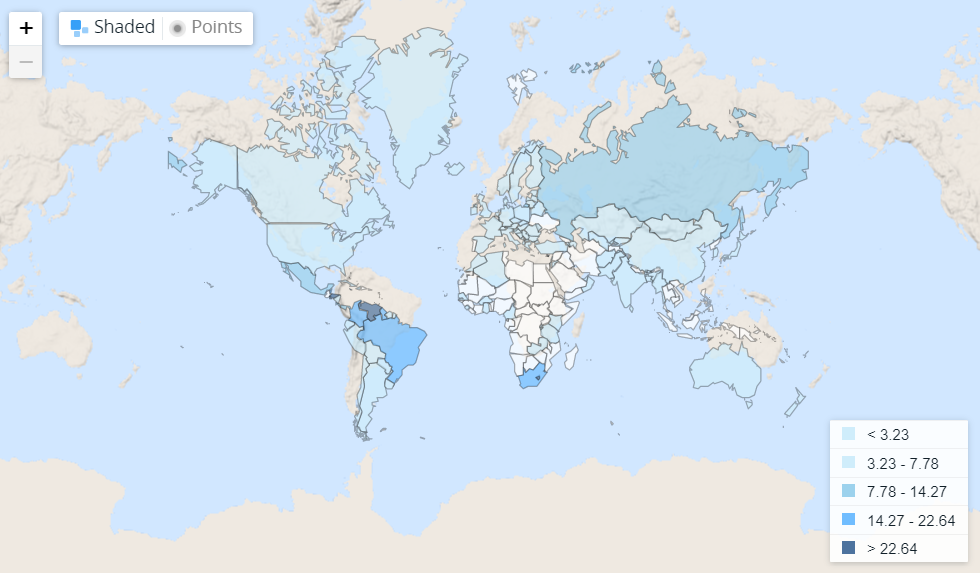
\includegraphics[scale=0.3]{homicides.png}
            \caption{Число убийств на 100000 человек за 2015 год --- данные Всемирного Банка).}
            
        \end{figure}
\end{frame}

\begin{frame}{2.Описание данных. Всемирный Банк}
\begin{figure} \label{hompic}
            \centering
            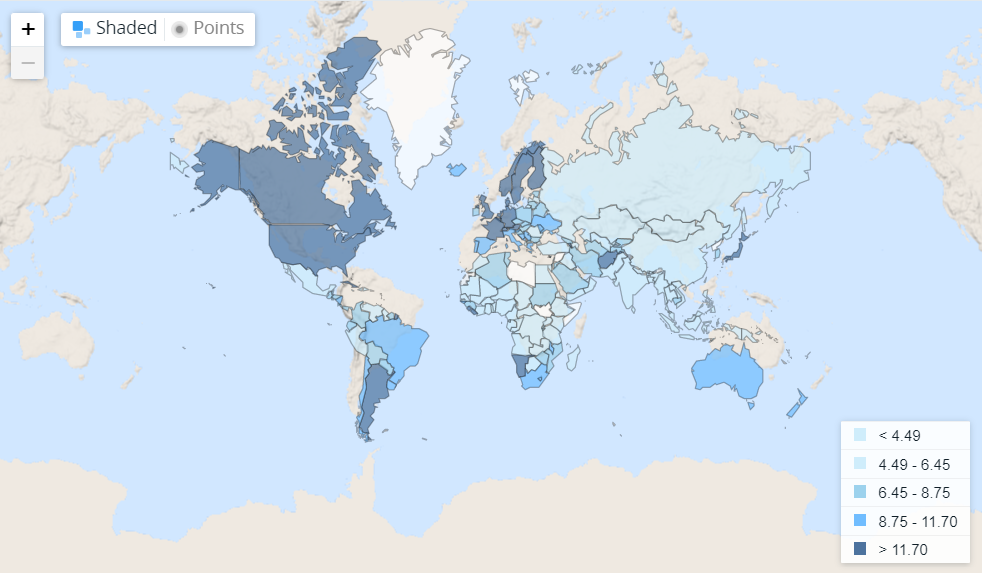
\includegraphics[scale=0.3]{medicine.png}
            \caption{Государственные расходы на медицину в процентах от ВВП  за 2015 год --- данные Всемирного Банка).}
            
        \end{figure}
\end{frame}

\begin{frame}{2.Описание данных. Всемирный Банк}
\begin{figure} \label{hompic}
            \centering
            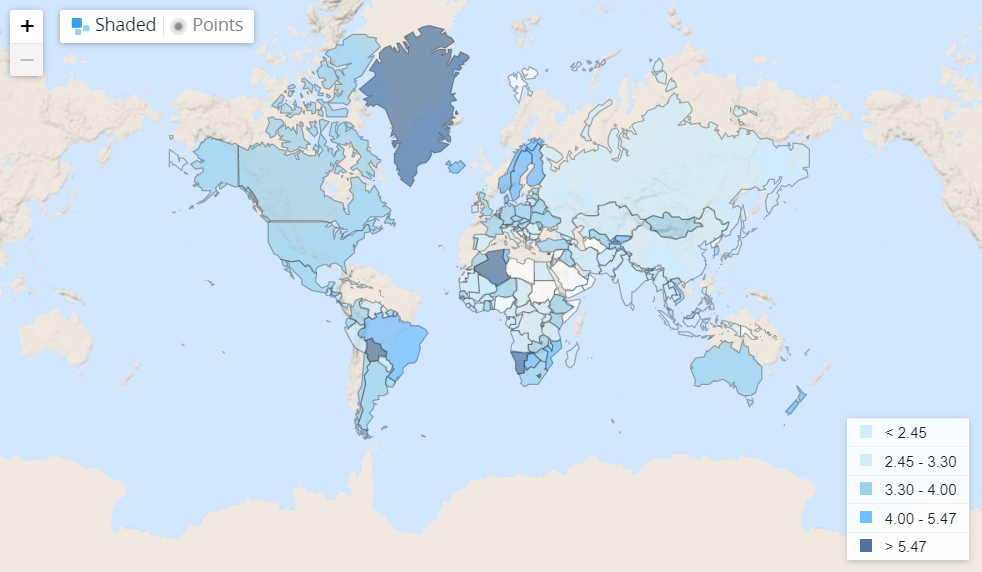
\includegraphics[scale=0.3]{education.png}
            \caption{Государственные расходы на образование в процентах от ВВП за 2015 год --- данные Всемирного Банка).}
            
        \end{figure}
\end{frame}

\begin{frame}{2.Описание данных. Всемирный Банк}
\begin{figure} \label{hompic}
            \centering
            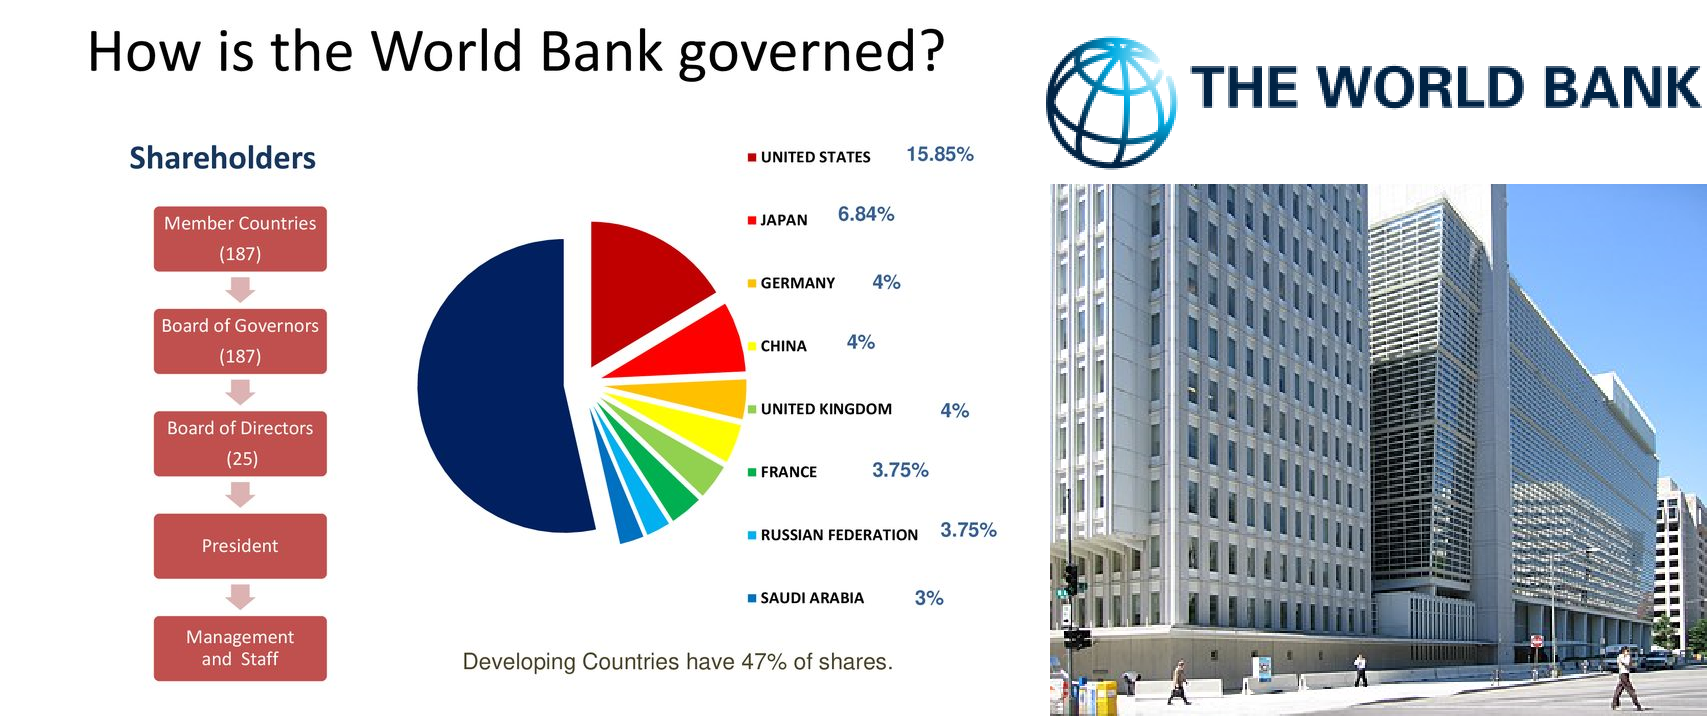
\includegraphics[scale=0.4]{Union4.png}
    \end{figure}
\end{frame}

\begin{frame}{Описание данных. World Happiness Report}
Всемирный доклад о счастье  — ежегодный доклад, публикуемый подразделением ООН по поиску решений стабильного развития (UN Sustainable Development Solutions Network). В июле 2011 года Генеральная Ассамблея ООН приняла резолюцию, призывающую страны — члены ООН, оценивать счастье своего народа и использовать его как ориентир в политике государства. 

\begin{figure} \label{hompic}
            \centering
            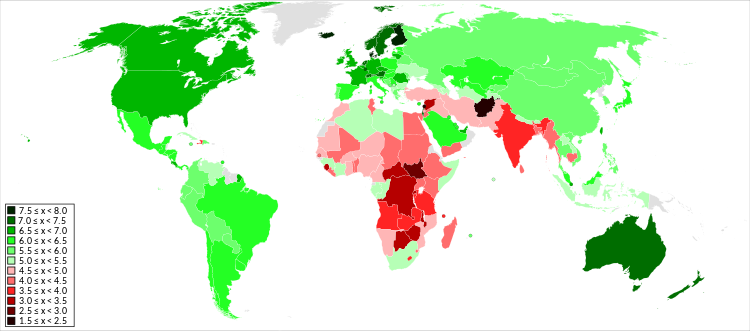
\includegraphics[scale=0.4]{Union5.png}
    \end{figure}

\end{frame}

\begin{frame}{3.Описание данных. Почему именно такие данные?}
\small
Как отмечалось во введении, экономика счастья — это весьма популярное направление исследований. Классиком этой области знаний считается Richard Easterlin, обративший внимание в статье 1 на связь доходов и счастья людей. Долгое время исследователь продвигал идею того, что уровень счастья людей не зависит от их доходов.
\hfill \break
\hfill \break
Однако, в этом вопросе всё не так однозначно. В 2010 году лауреаты премии Нобеля по экономике, Daniel Kahneman1 и Angus Deaton, опубликовали исследование 2, в котором, на примере США, показали, что счастье растёт вместе с доходами до определённого уровня, после которого рост, по меньшеё мере, очень существенно замедляется. Этот вопрос на самом деле невероятно важен и очень неочевиден, потому нам кажется целесообразным включение ВВП в той или иной форме в любые модели предсказания счастья. Впрочем, похоже, что это вполне соответствует общепринятому подходу к моделированию счастья: например, в 3 отмечалась важность роли ВВП. Этот показатель является регрессором в обеих рассматриваемых моделях. Причём, регрессию мы будем строить для логарифма подушевого ВВП по ППС, чтобы учесть эффект, описанный в начале настоящего
абзаца.

\end{frame}


\begin{frame}{3.Описание данных. Почему именно такие данные?}
Уровень безработицы также является одним из наиболее классических индикаторов положения дел в государстве. К тому же, есть серьёзные основания полагать, что он должен влиять на чувство удовлетворённости человека. Вопрос связи счастья и безработицы представляет самостоятельный интерес, поэтому существует немало статей, исследующих это, например, в публикации 6 было показано, что высокий уровень безработицы негативно влияет на счастье. В статье 8 этот тезис уже называется "общепринятым сама публикация посвящена исследованию некоторых деталей описываемого явления, кроме того, в ней можно найти ссылки на ещё большее число работ, всесторонне рассматривающих вопрос связи счастья и безработицы.
\hfill \break
\hfill \break

Что касается налоговой нагрузки, то здесь она, с одной стороны, является индикатором активности государственной социальной политики, а с другой, на самом деле может влиять на уровень счастья. Например, в статье 7 рассмотрена ситуация, в которой доказано влияние подоходного налога на уровень счастья.
\end{frame}

\begin{frame}{3.Описание данных. Почему именно такие данные?}
\small
С инфляцией всё гораздо менее очевидно. С одной стороны, не вызывает сомнений негативное отношение людей к инфляции (причины этого феномена исследуются, например, в статье 9). С другой стороны, центральные банки огромного количества стран осуществляют политику таргетирования инфляции, так что её величина является следствием положения дел в экономике, а не причиной. Счастье же населения, в данном контексте, зависит лишь от того, насколько грамотны решения регулятора. Тем не менее это очень значимый экономический показатель, поэтому мы включаем его в наши модели. Следующая категория объясняющих переменных связана со структурой государственного бюджета в двух наиболее значимых социальных сферах: в медицине (10) и в образовании (11).
\hfill \break
\hfill \break
Последняя категория переменных была внесена в рассмотрение в попытке описания как можно более разнообразных черт экономического и социального положения государства. Это преследует цель снижения эндогенности модели. Кроме того, мы рассматриваем решение о включении этих переменных в модель как попытку обнаружения новых показателей, значимо влияющих на уровень счастья.
\end{frame}

\begin{frame}{4.Модель с ’классическими’ объясняющими переменными}
   Целевой параметр описывается уравнением:
   \footnotesize{
        \begin{align*}
         Happiness = \beta_0 + \beta_1 \lg{GDP} + \beta_2 Unemployment + \beta_3 Tax + \beta_4 Inflation + \beta_5 Medicine + \beta_6 Education.
        \end{align*}
        }
    \normalsize
    Здесь $\lg{GDP}$ --- логарифм ВВП по ППС; $Unemployment $ --- уровень безработицы; $Tax $ -- налоговая нагрузка физических лиц. $Inflation $ --- инфляция; $Medicine $ --- государственные расходы на медицину; $Education $ --- государственные расходы на образование .
\hfill \break
\hfill \break
    Эта модель построена исходя из "рекомендаций" других статей. К тому же, каждую из переменных принято ассоциировать со счастьем, насчёт каждой из переменных проводились отдельные исследования.

\end{frame}

\begin{frame}{5.Модель со ’всеми’ переменными}
   Целевой параметр описывается уравнением:
   \footnotesize
        \begin{align*}
        Happiness = \beta_0 + \beta_1 \lg{GDP} + \beta_2 Unemployment + \beta_3 Tax + \beta_4 Inflation + \beta_5 Medicine + \beta_6 Education \\
            + \beta_7 Military + \beta_8 Savings + \beta_{9} AgeRatio + \beta_{10} Homicides + \beta_{11} Fertility.
        \end{align*}
    \normalsize

    Здесь $\lg{GDP}$ --- логарифм ВВП по ППС; $Unemployment$ --- уровень безработицы; $Tax$ -- налоговая нагрузка физических лиц. $Inflation$ --- инфляция; $Medicine$ --- государственные расходы на медицину; $Education$ --- государственные расходы на образование; $Military$ --- государственные военные расходы; $Savings$ --- валовая экономия; $Patents$ --- число зарегистрированных патентов по отношению к населению государства; $AgeRatio$ --- демографическая нагрузка; $Homicides$ --- число убийств на тысячу человек .
\hfill \break
\hfill \break
    В этой версии модели мы попытались рассмотреть как можно более разнообразные метрики благополучия страны.

\end{frame}

\begin{frame}{6.1.Результаты и их интерпретация}
   \begin{figure} \label{hompic}
            \centering
            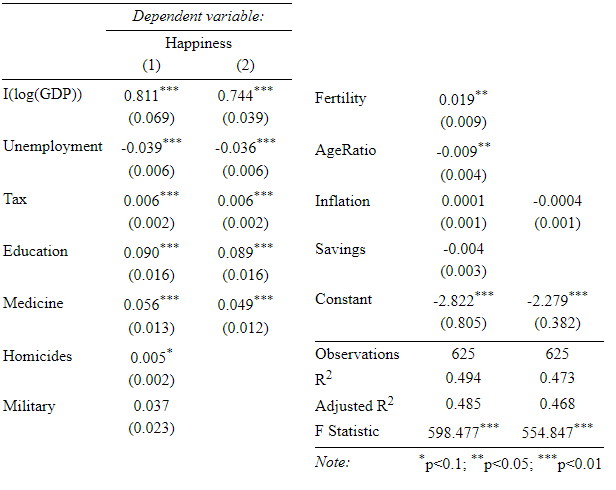
\includegraphics[scale=0.75]{UnionTable.png}
    \end{figure}

\end{frame}

\begin{frame}{6.Результаты и их интерпретация}
\small
   Результаты регрессионного анализа в рамках двух описанных выше моделей представлены в таблице (6.1 раздел) Они вполне предсказуемы: значимого эффекта у переменных вне рамок первой модели обнаружено не было, направление же влияния показателей на уровень счастья согласуется с результатами
   исследований (3 раздел). При этом, добавление новых переменных не привело к изменению коэффициентов при объясняющих переменных и их уровней значимости.
\hfill \break
\hfill \break
В результатах оценивания регрессии просматривается несколько интересных деталей.
\hfill \break
\hfill \break
Во-первых, не было обнаружено значимого явления инфляции на счастье. Отсутствие связи между этими показателями неочевидно и является довольно ценным аргументом в пользу рассуждений, высказанных в 3.
\hfill \break
\hfill \break
Во-вторых, не было обнаружено значимого влияния числа убийств (мы считаем это мерой криминализации общества). 
\end{frame}

\begin{frame}{6.Результаты и их интерпретация}
\small
Возможно, во-первых, больших проблем с учётом убийств не избежали даже развитые страны, а, во-вторых, в менее развитых странах, где криминогенная ситуация гораздо более тревожна, со сбором статистики подобного рода возникают очень существенные трудности, из-за чего de jure показатели развивающихся стран приближаются к de facto показателям развитых. Похоже, что такой эффект, в самом деле, может иметь место(см. 6.1).
\hfill \break
\hfill \break

В-третьих, не было обнаружено значимого влияния доли военных расходов на уровень
счастья. Это довольно примечательно, поскольку и рассуждения в духе ’высокие траты на оборону укрепляют в гражданах чувство безопасности и величия страны’ и таковые из серии ’военные траты есть, в сущности, сожжение денег, нужных для спасения жизней, во имя уничтожения таковых в неугодных государствах, такое мало кого может обрадовать’ кажутся довольно здравыми. Не исключено, впрочем, что оба эффекта имеют место и компенсируют друг друга.

\normalsize
\end{frame}

\begin{frame}{6.Результаты и их интерпретация}
Что касается незначимости остальных факторов, пожалуй, примечательной была бы ситуация их значимости. Они были добавлены в модель исключительно с целью проверки очевидных соображений и для лучшей эндогенности модели. Это небесполезно, ибо последние нередко оказываются не такими уж очевидными.
Как уже отмечалось выше, значимые коэффициенты не преподнесли сюрпризов. Примечательно, что коэффициент при доле трат на образование в полтора раза превосходит таковой при тратах на медицину. Впрочем, похоже, что это связано с тем, что доля образовательных расходов повсеместно меньше (см 6.1).
\end{frame}

\begin{frame}{7.Выводы}
   \small
   В статье исследуются две модели, описывающие зависимость счастья от некоторых макроэкономических показателей. Исследования подобных моделей помогают искать ответ на вопрос об этой связи и, на основании этого, строить рекомендации по осуществлению государственной политики и подтверждать (или опровергать) общепринятые идеи.
        \\
        Из ключевых результатов работы можно выделить следующее:
        \begin{itemize}
            \item Общепринятые и очевидные факты: экономическое развитие страны и увеличение доли бюджетных трат на образование значимо повышают уровень счастья граждан, увеличение же безработицы его уменьшает --- были подтверждены. Кроме того, были даны ссылки на публикации, более подробно исследующие эти темы.
            \item Увеличение налогов значимо повышает уровень счастья в модели.
            \item Не было выявлено значимого влияния инфляции, доли военных трат и демографической нагрузки на счастье.
            \item Не было выявлено значимого влияния числа убийств на счастье. Впрочем, похоже, что это свидетельствует о несостоятельности этой метрики, а не об отсутствии подобной связи.
        \end{itemize}
        

    \normalsize


\end{frame}

 \begin{frame}{8.Ссылки}
\tiny
 \begin{thebibliography}{100}
\bibitem{} \label{Easterlin}
            Easterlin R. A.
            Does Economic Growth Improve the Human Lot? Some Empirical Evidence.
            --- \textit{Nations and Households in Economic Growth}, 
            89-125, 1974.

            \bibitem{} \label{KahnemanDeaton}
            Kahneman D., Deaton A. 
            High income improves evaluation of life but not emotional well-being. 
            --- \textit{Proc Natl Acad Sci USA},
            \textbf{38}, 2010.

            \bibitem{} \label{DiTella}
            Di Tella R., MacCulloch R. J., Oswald A. J.
            The macroeconomics of happiness. 
           --- \textit{Review of Economics and Statistics}, 
            \textbf{85}, 1999. 

            \bibitem{} \label{Easterlin2}
            Easterlin R. A.
            Will Raising the Incomes of All Increase the Happiness of All?
            --- \textit{Journal of Economic Behaviour and Organization},
            \textbf{27}, 35-48, 1999. 

            \bibitem{} \label{Clark}
            Clark A. E., Oswald A. J.
            Unhappiness and Unemployment.
            --- \textit{Economic Journal}, 
            \textbf{104}, 648-659, 1994. 

            \bibitem{} \label{Winkelmann}
            Winkelmann L, Winkelmann R.
            Why are the unemployed so unhappy?
            --- \textit{Economica}, 
            \textbf{65}, 1-15, 1998. 

            \bibitem{} \label{tax}
            Hutchinson T., Ahmed I., Buryi P.
            Impact of income tax on happiness: evidence from the United States. 
            --- \textit{Applied Economics Letters}, 1-3.
            1-3, 2016.

            \bibitem{} \label{Clarkunemp}
            Clark A. E.
            A Note on Unhappiness and Unemployment Duration.
            --- \textit{IZA Discussion Paper No. 2406}, 
            2006. 
            
            \bibitem{} \label{Inflation}
            Shiller J. R.
            Why Do People Dislike Inflation?
            --- \textit{NBER Working Paper}, 
            \textbf{5539}, 1996. 

            \bibitem{} \label{medicine}
            Dfarhud D., Maryam M., Khanahmadi M. 
            Happiness & Health: The Biological Factors-Systematic Review Article.
            --- \textit{Iranian Journal of Public Health}, 
            \textbf{43}, 1468-1477, 2014. 

            \bibitem{} \label{Education}
            Satoshi Araki.
            Does Education Make People Happy? Spotlighting the Overlooked Societal Condition.
            --- \textit{Journal of Happiness Studies}, 
            \textbf{23}, 587-629, 2021.
    \end{thebibliography}
 \end{frame}

 
\end{document}